% Exercises for Lesson 10: TikZ Graphics Basics
% Topic: LaTeX
% Solutions to practice problems from the lesson.
% Compile: pdflatex exercises/LaTeX/10_tikz_basics.tex

\documentclass[12pt, a4paper]{article}
\usepackage[utf8]{inputenc}
\usepackage[T1]{fontenc}
\usepackage{amsmath, amssymb}
\usepackage{tikz}
\usetikzlibrary{arrows.meta, positioning, shapes.geometric, calc}

\title{Exercises for Lesson 10: TikZ Graphics Basics}
\author{Study Project}
\date{}

\begin{document}
\maketitle

% === Exercise 1: Basic Shapes ===
% Problem: Red circle, blue rectangle, green triangle, yellow ellipse, labeled.

\section*{Exercise 1: Basic Shapes}

\begin{center}
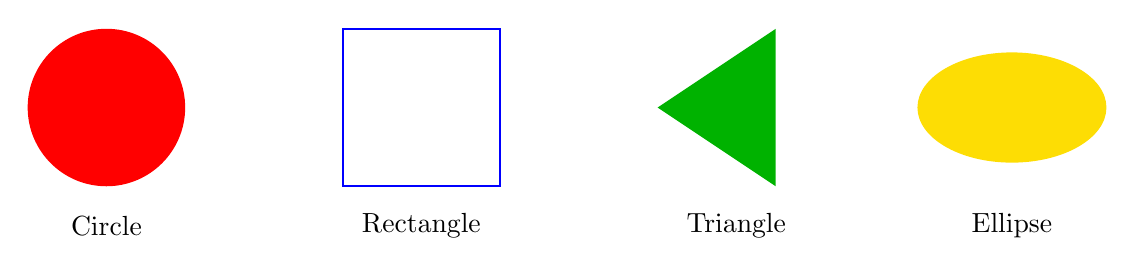
\begin{tikzpicture}
  % Red filled circle
  \fill[red] (0,0) circle (1cm);
  \node at (0,-1.5) {Circle};

  % Blue outlined rectangle
  \draw[blue, thick] (3,-1) rectangle (5,1);
  \node at (4,-1.5) {Rectangle};

  % Green filled triangle
  \fill[green!70!black] (7,0) -- (8.5,1) -- (8.5,-1) -- cycle;
  \node at (8,-1.5) {Triangle};

  % Yellow filled ellipse
  \fill[yellow!80!orange] (11.5,0) ellipse (1.2cm and 0.7cm);
  \node at (11.5,-1.5) {Ellipse};
\end{tikzpicture}
\end{center}

% === Exercise 2: Coordinate Systems ===
% Problem: 5 Cartesian points, 5 polar points, connect, label.

\section*{Exercise 2: Coordinate Systems}

\begin{center}
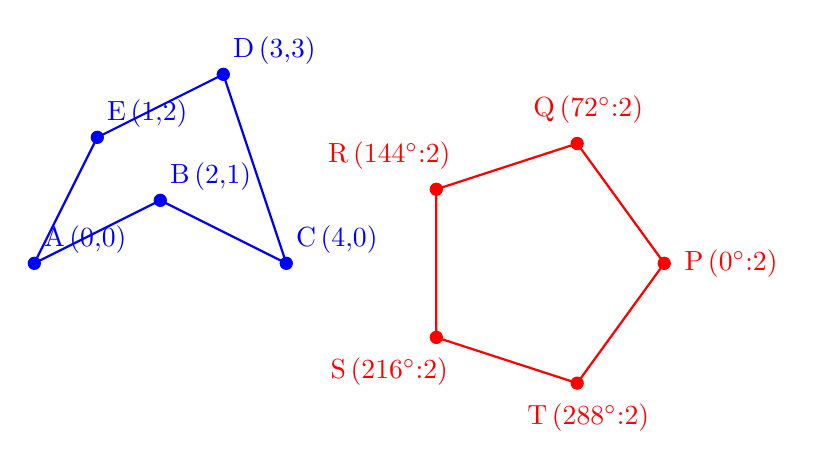
\begin{tikzpicture}[scale=0.8]
  % Cartesian points
  \foreach \x/\y/\name in {0/0/A, 2/1/B, 4/0/C, 3/3/D, 1/2/E} {
    \fill[blue] (\x,\y) circle (3pt) node[above right] {\name\,(\x,\y)};
  }
  \draw[blue, thick] (0,0) -- (2,1) -- (4,0) -- (3,3) -- (1,2) -- cycle;

  % Polar points (shifted right)
  \begin{scope}[xshift=8cm]
    \foreach \angle/\radius/\name in {
      0/2/P, 72/2/Q, 144/2/R, 216/2/S, 288/2/T} {
      \fill[red] (\angle:\radius) circle (3pt)
        node[anchor=\angle+180, outer sep=4pt]
        {\name\,($\angle^\circ$:$\radius$)};
    }
    \draw[red, thick]
      (0:2) -- (72:2) -- (144:2) -- (216:2) -- (288:2) -- cycle;
  \end{scope}
\end{tikzpicture}
\end{center}

% === Exercise 3: Line Styles ===
% Problem: Legend of thicknesses, dash patterns, colors.

\section*{Exercise 3: Line Styles}

\begin{center}
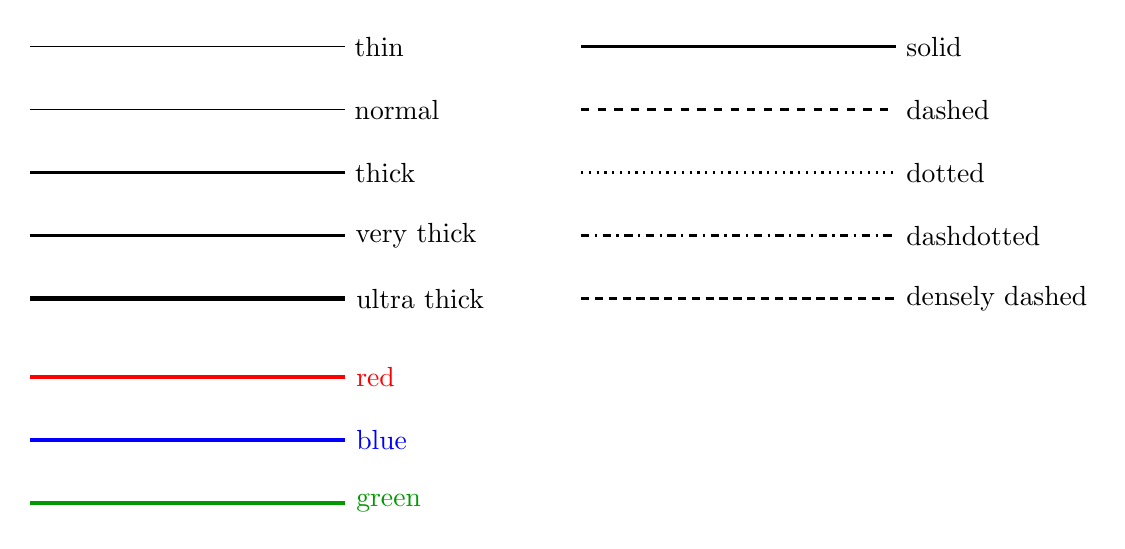
\begin{tikzpicture}
  % Thickness variations
  \draw[thin]       (0, 4) -- (4, 4) node[right] {thin};
  \draw[]           (0, 3.2) -- (4, 3.2) node[right] {normal};
  \draw[thick]      (0, 2.4) -- (4, 2.4) node[right] {thick};
  \draw[very thick] (0, 1.6) -- (4, 1.6) node[right] {very thick};
  \draw[ultra thick] (0, 0.8) -- (4, 0.8) node[right] {ultra thick};

  % Dash patterns
  \draw[thick, solid]       (7, 4) -- (11, 4) node[right] {solid};
  \draw[thick, dashed]      (7, 3.2) -- (11, 3.2) node[right] {dashed};
  \draw[thick, dotted]      (7, 2.4) -- (11, 2.4) node[right] {dotted};
  \draw[thick, dashdotted]  (7, 1.6) -- (11, 1.6) node[right] {dashdotted};
  \draw[thick, densely dashed] (7, 0.8) -- (11, 0.8) node[right] {densely dashed};

  % Color variations
  \draw[ultra thick, red]    (0, -0.2) -- (4, -0.2) node[right] {red};
  \draw[ultra thick, blue]   (0, -1.0) -- (4, -1.0) node[right] {blue};
  \draw[ultra thick, green!60!black] (0, -1.8) -- (4, -1.8)
    node[right] {green};
\end{tikzpicture}
\end{center}

% === Exercise 4: Nodes and Anchors ===
% Problem: Central node, 8 smaller nodes at anchors, connections, labels.

\section*{Exercise 4: Nodes and Anchors}

\begin{center}
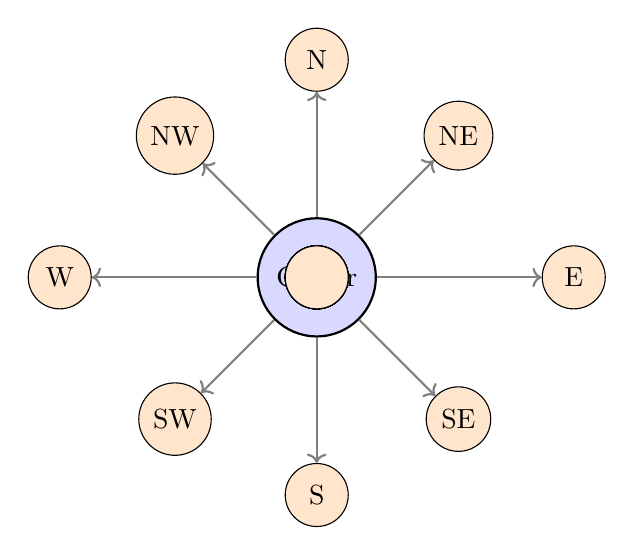
\begin{tikzpicture}[
  center node/.style={draw, circle, minimum size=1.5cm, thick, fill=blue!15},
  anchor node/.style={draw, circle, minimum size=0.8cm, fill=orange!20}
]
  \node[center node] (center) {Center};

  \foreach \anchor/\label in {
    north/N, south/S, east/E, west/W,
    north east/NE, north west/NW, south east/SE, south west/SW} {
    \node[anchor node] (\anchor) at (center.\anchor |- {0,0} -| {0,0}) {};
  }

  % Position anchor nodes at distance from center
  \node[anchor node] (N)  at ([yshift=2cm]center.north)      {N};
  \node[anchor node] (S)  at ([yshift=-2cm]center.south)     {S};
  \node[anchor node] (E)  at ([xshift=2.5cm]center.east)     {E};
  \node[anchor node] (W)  at ([xshift=-2.5cm]center.west)    {W};
  \node[anchor node] (NE) at ([shift={(1.8cm,1.8cm)}]center) {NE};
  \node[anchor node] (NW) at ([shift={(-1.8cm,1.8cm)}]center){NW};
  \node[anchor node] (SE) at ([shift={(1.8cm,-1.8cm)}]center){SE};
  \node[anchor node] (SW) at ([shift={(-1.8cm,-1.8cm)}]center){SW};

  % Connect each to center
  \foreach \anchor in {N, S, E, W, NE, NW, SE, SW} {
    \draw[->, thick, gray] (center) -- (\anchor);
  }
\end{tikzpicture}
\end{center}

% === Exercise 5: Simple Flowchart ===
% Problem: Tea-making flowchart with start, decision, processes, end.

\section*{Exercise 5: Flowchart -- Making Tea}

\begin{center}
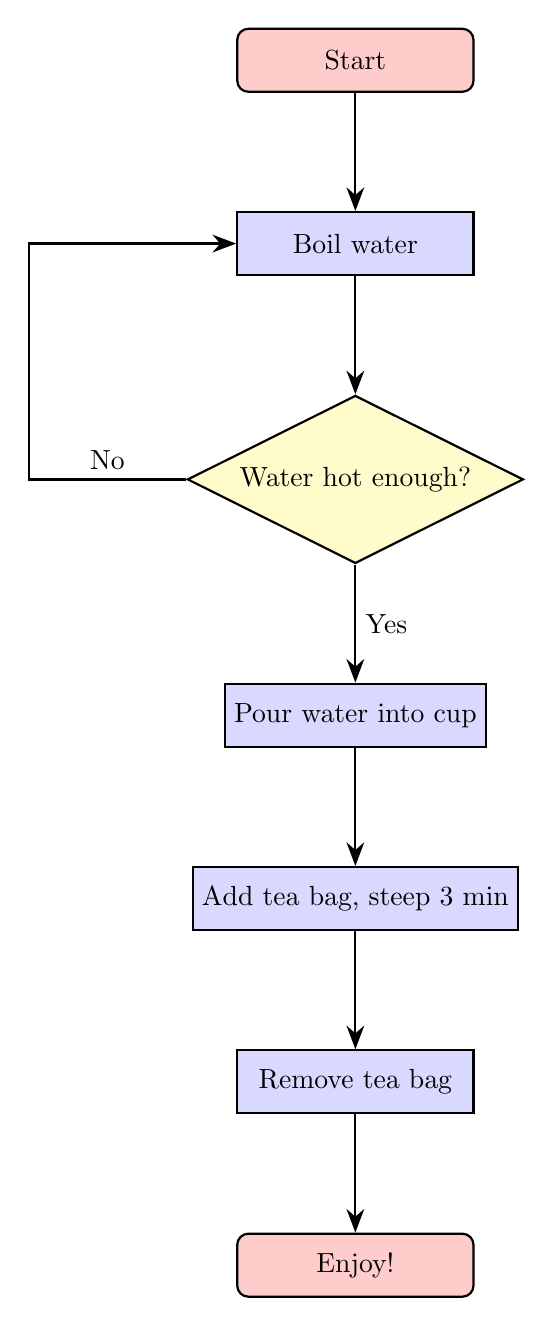
\begin{tikzpicture}[
  node distance=1.5cm,
  startstop/.style={rectangle, rounded corners, draw, thick,
    fill=red!20, minimum width=3cm, minimum height=0.8cm},
  process/.style={rectangle, draw, thick, fill=blue!15,
    minimum width=3cm, minimum height=0.8cm},
  decision/.style={diamond, draw, thick, fill=yellow!20,
    minimum width=2cm, minimum height=1cm, aspect=2},
  arrow/.style={-{Stealth[length=3mm]}, thick}
]
  \node[startstop] (start) {Start};
  \node[process, below=of start] (boil) {Boil water};
  \node[decision, below=of boil] (hot) {Water hot enough?};
  \node[process, below=of hot] (pour) {Pour water into cup};
  \node[process, below=of pour] (steep) {Add tea bag, steep 3 min};
  \node[process, below=of steep] (remove) {Remove tea bag};
  \node[startstop, below=of remove] (end) {Enjoy!};

  \draw[arrow] (start) -- (boil);
  \draw[arrow] (boil) -- (hot);
  \draw[arrow] (hot) -- node[right] {Yes} (pour);
  \draw[arrow] (hot.west) -- ++(-2,0) node[above, midway] {No}
    |- (boil.west);
  \draw[arrow] (pour) -- (steep);
  \draw[arrow] (steep) -- (remove);
  \draw[arrow] (remove) -- (end);
\end{tikzpicture}
\end{center}

% === Exercise 6: Grid and Axes ===
% Problem: Grid, labeled axes with arrows, tick marks, labels, origin.

\section*{Exercise 6: Grid and Axes}

\begin{center}
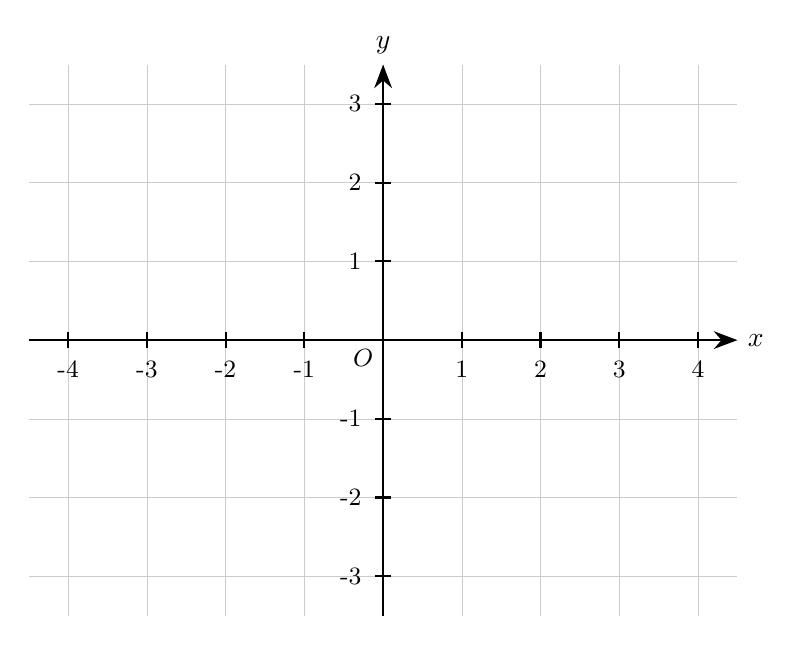
\begin{tikzpicture}
  % Grid
  \draw[help lines, gray!40] (-4.5,-3.5) grid (4.5,3.5);

  % Axes
  \draw[-{Stealth[length=3mm]}, thick] (-4.5,0) -- (4.5,0) node[right] {$x$};
  \draw[-{Stealth[length=3mm]}, thick] (0,-3.5) -- (0,3.5) node[above] {$y$};

  % Tick marks and labels on x-axis
  \foreach \x in {-4,-3,-2,-1,1,2,3,4} {
    \draw[thick] (\x, -0.1) -- (\x, 0.1);
    \node[below, font=\small] at (\x, -0.15) {\x};
  }

  % Tick marks and labels on y-axis
  \foreach \y in {-3,-2,-1,1,2,3} {
    \draw[thick] (-0.1, \y) -- (0.1, \y);
    \node[left, font=\small] at (-0.15, \y) {\y};
  }

  % Origin
  \node[below left, font=\small] at (0,0) {$O$};
\end{tikzpicture}
\end{center}

% === Exercise 7: Filled Shapes ===
% Problem: 3 overlapping circles with transparency, gradient rectangle,
% shape with different fill and draw.

\section*{Exercise 7: Filled Shapes with Transparency}

\begin{center}
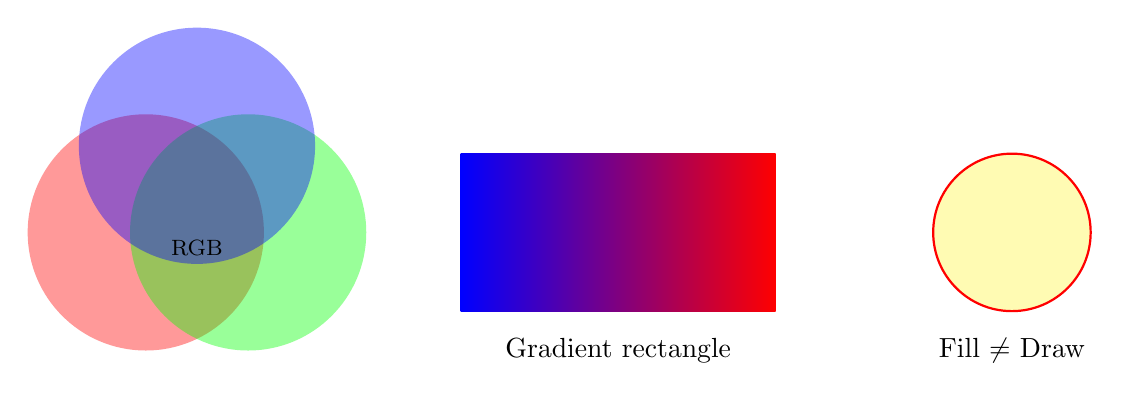
\begin{tikzpicture}
  % Three overlapping circles
  \fill[red, opacity=0.4]   (0,0) circle (1.5cm);
  \fill[green, opacity=0.4] (1.3,0) circle (1.5cm);
  \fill[blue, opacity=0.4]  (0.65,1.1) circle (1.5cm);
  \node at (0.65,-0.2) {\footnotesize RGB};

  % Gradient rectangle
  \shade[left color=blue, right color=red] (4,-1) rectangle (8,1);
  \node at (6,-1.5) {Gradient rectangle};

  % Different fill and draw
  \filldraw[draw=red, thick, fill=yellow!30] (11,0) circle (1cm);
  \node at (11,-1.5) {Fill $\neq$ Draw};
\end{tikzpicture}
\end{center}

% === Exercise 8: Path Drawing -- House ===
% Problem: House using \draw paths, cycle, colors.

\section*{Exercise 8: House Drawing}

\begin{center}
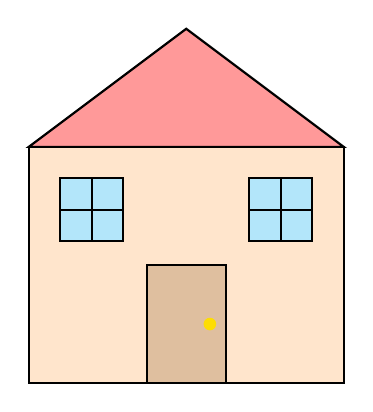
\begin{tikzpicture}[thick]
  % House body
  \draw[fill=orange!20] (0,0) rectangle (4,3);

  % Roof (triangle)
  \draw[fill=red!40] (0,3) -- (2,4.5) -- (4,3) -- cycle;

  % Door
  \draw[fill=brown!50] (1.5,0) rectangle (2.5,1.5);
  \fill[yellow!80!orange] (2.3,0.75) circle (0.08);

  % Windows
  \draw[fill=cyan!30] (0.4,1.8) rectangle (1.2,2.6);
  \draw (0.8,1.8) -- (0.8,2.6);
  \draw (0.4,2.2) -- (1.2,2.2);

  \draw[fill=cyan!30] (2.8,1.8) rectangle (3.6,2.6);
  \draw (3.2,1.8) -- (3.2,2.6);
  \draw (2.8,2.2) -- (3.6,2.2);
\end{tikzpicture}
\end{center}

% === Exercise 9: Bezier Curves ===
% Problem: Wave pattern, control points as circles, connecting lines.

\section*{Exercise 9: B\'{e}zier Curves}

\begin{center}
\begin{tikzpicture}
  % Define points
  \coordinate (A) at (0,0);
  \coordinate (CP1) at (1,2);
  \coordinate (B) at (3,0);
  \coordinate (CP2) at (5,-2);
  \coordinate (C) at (7,0);
  \coordinate (CP3) at (9,2);
  \coordinate (D) at (11,0);

  % Draw Bezier wave
  \draw[thick, blue]
    (A) .. controls (CP1) and ($(B)-(1,2)$) ..
    (B) .. controls ($(B)+(1,-2)$) and ($(C)-(1,2)$) ..
    (C) .. controls ($(C)+(1,2)$) and ($(D)-(1,2)$) ..
    (D);

  % Control points
  \foreach \point/\label in {CP1/CP1, CP2/CP2, CP3/CP3} {
    \fill[red] (\point) circle (3pt);
    \node[above, red, font=\small] at (\point) {\label};
  }

  % Path points
  \foreach \point/\label in {A/A, B/B, C/C, D/D} {
    \fill[black] (\point) circle (3pt);
    \node[below, font=\small] at (\point) {\label};
  }

  % Lines from path points to control points
  \draw[thin, gray, dashed] (A) -- (CP1);
  \draw[thin, gray, dashed] (C) -- (CP3);
\end{tikzpicture}
\end{center}

% === Exercise 10: Network Diagram ===
% Problem: 5 computers, 1 router, 1 server, connections, labels, colors.

\section*{Exercise 10: Network Diagram}

\begin{center}
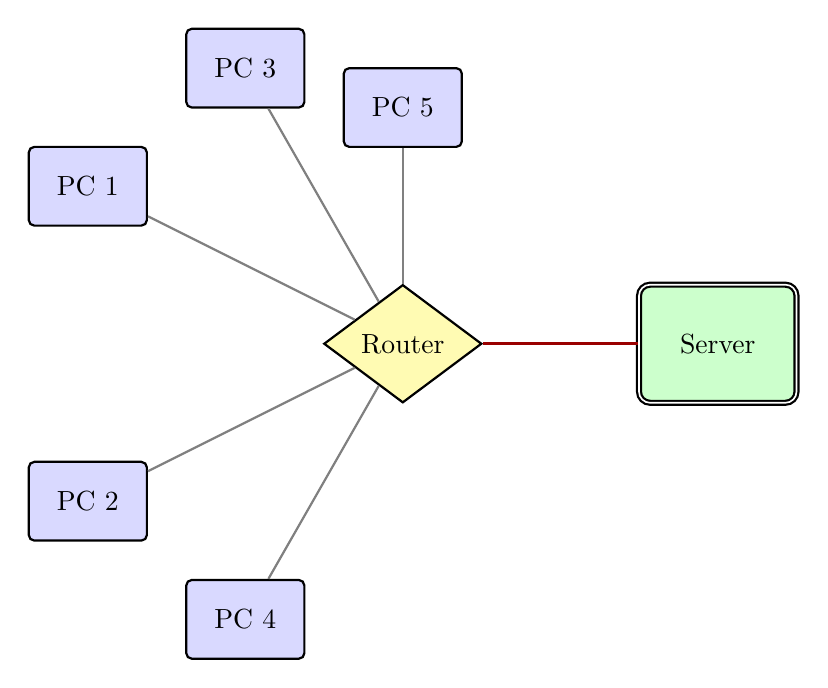
\begin{tikzpicture}[
  computer/.style={rectangle, draw, thick, fill=blue!15,
    minimum width=1.5cm, minimum height=1cm, rounded corners=2pt},
  router/.style={diamond, draw, thick, fill=yellow!30,
    minimum width=1.5cm, minimum height=1.5cm, aspect=1.5},
  server/.style={rectangle, draw, thick, fill=green!20,
    minimum width=2cm, minimum height=1.5cm, rounded corners=4pt,
    double},
  conn/.style={thick, gray}
]
  % Router at center
  \node[router] (R) at (0,0) {Router};

  % Computers around the router
  \node[computer] (C1) at (-4, 2)  {PC 1};
  \node[computer] (C2) at (-4,-2)  {PC 2};
  \node[computer] (C3) at (-2, 3.5){PC 3};
  \node[computer] (C4) at (-2,-3.5){PC 4};
  \node[computer] (C5) at (0, 3)   {PC 5};

  % Server
  \node[server] (S) at (4, 0) {Server};

  % Connections
  \foreach \c in {C1, C2, C3, C4, C5} {
    \draw[conn] (\c) -- (R);
  }
  \draw[conn, very thick, red!60!black] (R) -- (S);
\end{tikzpicture}
\end{center}

\end{document}
